\documentclass[../Kamil_Kowalewski_Main.tex]{subfiles}

\begin{document} {

    Celem przyświecającym autorowi niniejszej pracy magisterskiej było stworzenie
    środowiska eksperymentalnego opierającego się na standardach oraz technologiach
    uznawanych przez ekspertów jako wiodące. Co więcej, niezwykle ważne również było
    korzystanie z~narzędzi w~pełni darmowych lub otwartoźródłowych, aby w~przyszłości
    odwzorowanie badań było zadaniem, które nie będzie sprawiać problemów.

    \section{Implementacja programu}
    \label{chapter4:srodowisko_eksperymentalne:impl_programu} {

        \subsection{Uzasadnienie wyboru języka programowania}
        \label{chapter4:srodowisko_eksperymentalne:impl_programu:jezyk} {
            Autor zdecydował się na wykorzystanie języka programowania
            Python\cite{website:python} ze względu na jego popularność w~dziedzinach
            informatyki związanych z~uczeniem maszynowym, analizą danych czy też data
            science. Jest to technologia niezwykle wygodna oraz przystępna do
            przetwarzania oraz analizy danych, również tych złożonych. Jej rozwój
            następują w~sposób dynamiczny, lecz zrównoważony, dzięki czemu jego
            wykorzystywanie oraz utrzymanie projektu napisanego we właśnie tej
            technologii nie stanowi problemu. Jednymi z~głównych sponsorów są takie
            przedsiębiorstwa jak Google\cite{website:google} czy
            Microsoft\cite{website:microsoft} co daje wysoki stopień pewności
            systematycznych aktualizacji, naprawy odnalezionych luk bezpieczeństwa oraz
            błędów w~oprogramowaniu.
        }

        \subsection{Wykorzystane biblioteki programistyczne}
        \label{chapter4:srodowisko_eksperymentalne:impl_programu:bib} {
            Aby efektywnie wykorzystać potencjał języka Python oraz jego możliwości,
            zostały wykorzystane popularne biblioteki programistyczne. Należą do nich
            chociażby NumPy\cite{website:numpy} lub Pandas\cite{website:pandas} oraz
            biblioteki opisane poniżej w~ramach tej sekcji. Są one przede wszystkim
            bardzo znane, posiadają świetną dokumentację techniczną. Poziom
            i~dokładność otestowania jest bardzo wysoki. Co więcej, tak samo, jak język
            programowania Python, są sponsorowane przez wiodące firmy z~sektora IT.
            Dzięki temu wszelkie błędy są bardzo szybko naprawiane, a~samo wydanie nowej
            wersji poprzedzają dogłębne testy.

            \subsubsection{Biblioteka NumPy}
            \label{chapter4:srodowisko_eksperymentalne:impl_programu:bib:numpy} {
                Pierwszą ze wspomnianych bibliotek jest biblioteka NumPy. Jej główną
                funkcjonalnością jest N-wymiarowa tablica. Dzięki niej w~bardzo
                przystępny sposób istnieje możliwość przechowywania danych w~postaci
                macierzowej, które są tak popularne w~przypadku zagadnień związanych
                z~uczeniem maszynowym czy analizą danych. Oczywiście \textit{N} jest
                parametrem, którego dolną granicą jest wartość \textit{1}, natomiast
                górna granica to fizyczne ograniczenia sprzętowe. Dla przykładu tablica
                może być \textit{100} wymiarowa, jeśli jest potrzeba przechowywania
                takich danych. Warto dodać, że biblioteka ta zapewnia bardzo duży zbiór
                operacji matematycznych, jakie można wykonywać oraz numeryczne narzędzia
                obliczeniowe takie jak transformaty Fouriera, czy funkcje wymagane do
                algebry liniowej. Całość zwieńcza fakt, iż rdzeń biblioteki został
                zaimplementowany w~dobrze zoptymalizowanym kodzie napisanym w~języku
                programowania \textit{C}. Na listingu
                \ref{lst:chapter4:srodowisko_eksperymentalne:impl_programu:bib:numpy}
                został przedstawiony przykład użycia biblioteki Numpy.

                \begin{code}[H]
                    \lstinputlisting{../listing/chapter4/numpy.txt}
                    \caption
                    [Przykładowe użycie biblioteki NumPy]
                    {Przykładowe użycie biblioteki NumPy}
                    \label
                    {lst:chapter4:srodowisko_eksperymentalne:impl_programu:bib:numpy}
                \end{code}
            }

            \subsubsection{Biblioteka Pandas}
            \label{chapter4:srodowisko_eksperymentalne:impl_programu:bib:pandas} {
                Biblioteka Pandas również ma za zadanie zapewniać infrastrukturę do
                przechowywania danych. W~jej przypadku głównym obiektem jest
                \textit{DataFrame}. Zapewnia on możliwość przechowywania oraz
                manipulacji danymi. Jest w~nim również zintegrowane indeksowanie.
                Biblioteka ta jest szczególnie wygodna do operowania na danych
                dostarczonych w~formatach \textit{.csv}, \textit{.tsv}, czy też
                \textit{.xlsx} oraz wielu innych, które są mniej popularne. Dla każdego
                typu jest przygotowana w~bibliotece określona metoda do wygodnego
                wczytywania zbioru danych. Są to np. \textit{pd.read\_csv()}, czy też
                \textit{pd.read\_excel()}, które zwracają wspomniany wcześniej obiekt
                \textit{DataFrame}. Dostępnych jest wiele operacji, jakie możemy na nim
                wykonywać poprzez użycie dostarczonych w~bibliotece funkcji. Założenia
                przyświecające autorom były takie, aby funkcjonalności były bardzo
                intuicyjne. Wszystkie operacje są dokonywane w~sposób deklaratywny,
                jest to mocno zbliżone do kwerend wykonywanych w~języku SQL
                (ang. Structured Query Language). Co więcej, dostępne są też analogiczne
                funkcję jak w~SQL, a~mianowicie \textit{count()}, \textit{groupby()},
                \textit{join()}. Dostarczane są również funkcje przeznaczone stricte do
                zadań z~tematyki Data Science jak imputacje brakujących danych,
                usuwanie pustych rekordów, czy też konwersje do oczekiwane formatu np.
                zamiana dokładnej daty na porę roku co daje możliwość uzyskania
                lepszych wyników po dokonaniu analizy danych. Na listingu
                \ref{lst:chapter4:srodowisko_eksperymentalne:impl_programu:bib:pandas}
                został przedstawiony przykład użycia biblioteki Pandas.

                \begin{code}[H]
                    \lstinputlisting{../listing/chapter4/pandas.txt}
                    \caption
                    [Przykładowe użycie biblioteki Pandas]
                    {Przykładowe użycie biblioteki Pandas}
                    \label
                    {lst:chapter4:srodowisko_eksperymentalne:impl_programu:bib:pandas}
                \end{code}
            }

            \subsubsection{Biblioteka Matplotlib}
            \label{chapter4:srodowisko_eksperymentalne:impl_programu:bib:} {
                Biblioteka Matplotlib\cite{website:matplotlib} należy również do grona
                najbardziej popularnych oraz wręcz bazowych narzędzi w~rękach
                programisty języka Python. Zapewnia ona możliwość bardzo zaawansowanej
                wizualizacji danych przechowywanych we wcześniej wspomnianych
                bibliotekach, a~mianowicie NumPy oraz Pandas. Samo jej podstawowe użycie
                jest niezwykle łatwe oraz intuicyjne, dzięki czemu stała się wręcz
                podstawowym narzędziem do przedstawiania uzyskanych wyników. Jest ona
                oczywiście w~pełni darmowa oraz ciągle rozwijana w~dynamiczny sposób
                więc jej wykorzystanie nie niesie za sobą niebezpieczeństwa utraty
                wsparcia po pewnym czasie.

                \begin{code}[H]
                    \lstinputlisting{../listing/chapter4/matplotlib.txt}
                    \caption
                    [Przykładowe użycie biblioteki matplotlib]
                    {Przykładowe użycie biblioteki matplotlib}
                    \label
                    {lst:chapter4:srodowisko_eksperymentalne:impl_programu:bib:matplotlib}
                \end{code}
            }

            \subsubsection{Biblioteka scikit-learn}
            \label{chapter4:srodowisko_eksperymentalne:impl_programu:bib:sklearn} {
                Kolejną biblioteką z~wymienianych jest scikit-learn\cite{website:sklearn}.
                Aby zapewnić deklarowane przez twórców funkcjonalności wykorzystuje ona
                w~biblioteki takie jak NumPy oraz Pandas, które są de facto standardem
                i~wykorzystywane są przez wiele innych bibliotek zapewniających
                implementacje różnych algorytmów uczenia maszynowego. Sam scikit-learn
                należy właśnie do grupy bibliotek zapewniających zróżnicowane algorytmy
                uczenia maszynowego. Są one pogrupowane ze względu na rodzaj, można
                wyróżnić następujące grupy algorytmów klasyfikacji, klasteryzacji
                (grupowania), regresji, redukcji wymiarowości oraz dotyczące
                preprocessingu. Samo wykorzystanie dostępnych funkcji oraz metod jest
                bardzo proste oraz intuicyjne ze względu na spójny interfejs
                prezentowany przez klasy oraz bardzo sensownie dobrane domyślne
                wartości. Dzięki temu nawet bez dogłębnych badań, w~krótkim czasie można
                uzyskiwać zadowalające wyniki. Co warto dodać dostarczana jest świetna
                dokumentacja, w~której są również przykłady jak stosować konkretne
                metody i~algorytmy, ich podstawy teoretyczne z bardzo dobrą
                wizualizacją. Wspierają to szybszy rozwój osoby z~niej korzystającej oraz
                częściowo eliminuje możliwość dobrania złego algorytmu do problemu. Na
                listingu
                \ref{lst:chapter4:srodowisko_eksperymentalne:impl_programu:bib:sklearn}
                został przedstawiony przykład użycia biblioteki scikit-learn.

                \begin{code}[H]
                    \lstinputlisting{../listing/chapter4/sklearn.txt}
                    \caption
                    [Przykładowe użycie biblioteki scikit-learn]
                    {Przykładowe użycie biblioteki scikit-learn}
                    \label
                    {lst:chapter4:srodowisko_eksperymentalne:impl_programu:bib:sklearn}
                \end{code}
            }

            \subsubsection{Biblioteka NLTK}
            \label{chapter4:srodowisko_eksperymentalne:impl_programu:bib:nltk} {
                Biblioteka NLTK\cite{website:nltk} zapewnia możliwość przetwarzania
                oraz analizy języka naturalnego, stąd też jej nazwa (ang. Natural
                Language Toolkit). Dzięki niej dostępne są operacje wstępnego
                przetwarzania takie jak tokenizacji, usuwanie słów występujących w~stop
                liście (ang. stop words), przeprowadzanie stemizacji (ang. stemming) lub
                lematyzacji (ang. lemmatization). Co więcej, można dokonywać wykrywania
                języka na podstawie podane fragmentu tekstu, czy też analizy sentymentu
                danej wypowiedzi lub tekstu. Informacją zwrotną analizy sentymentu
                jest stopień w~jakim jest ona pozytywna, neutralna lub też negatywna.
                Co ciekawe jest udostępniona możliwość graficznej demonstracji np.
                analizy składniowej bądź dokonania tłumaczenia z~konkretnego języka
                na wybrany.
            }

            \subsubsection{Biblioteka NRCLex}
            \label{chapter4:srodowisko_eksperymentalne:impl_programu:bib:nrclex} {
                Biblioteka NRCLex\cite{website:nrclex} zapewnia jeszcze bardziej
                rozbudowaną analizę sentymentu. Na podstawie słów określa emocje
                zawarte w~tekście, poprzez zwrócenie wartości od \textit{0} do
                \textit{1} w~każdej z~kategorii przedstawionych poniżej:
                \begin{itemize}[noitemsep,topsep=1pt]
                    \item strach (ang. fear)
                    \item gniew (ang. anger)
                    \item oczekiwanie (ang. anticipation)
                    \item zaufanie (ang. trust)
                    \item niespodzianka (ang. surprise)
                    \item pozytywność (ang. positive)
                    \item negatywność (ang. negative)
                    \item smutek (ang. sadness)
                    \item obrzydzenia (ang. disgust)
                    \item radość (ang. joy)
                \end{itemize}

                Co warto wspomnieć, suma wartości we wszystkich kategoriach jest równa
                \textit{1}. Dodatkowo są zapewnione funkcjonalności dzielenia na słowa
                czy też zdania, natomiast zbiory danych do określania emocji są
                wykorzystywane z~biblioteki NLTK opisanej w~sekcji
                \ref{chapter4:srodowisko_eksperymentalne:impl_programu:bib:nltk}.
            }

        }

        \subsection{Struktura modułów i komponentów}
        \label{chapter4:srodowisko_eksperymentalne:impl_programu:struktura} {
            Program implementujący metodę przedstawioną w~sekcji
            \ref{chapter3:metoda:warianty_metody}, został przygotowany zgodnie
            z~popularnymi i~uznawanymi przez wiele osób \textit{dobrymi praktykami}.
            Autor zdecydował się wydzielić cztery pakiety. Są to \textit{model},
            \textit{service}, \textit{interface} oraz \textit{exception}, przedstawione
            odpowiednio na rysunkach
            \ref{fig:chapter4:srodowisko_eksperymentalne:model_package},
            \ref{fig:chapter4:srodowisko_eksperymentalne:service_package},
            \ref{fig:chapter4:srodowisko_eksperymentalne:inteface_package},
            \ref{fig:chapter4:srodowisko_eksperymentalne:exception_package}.
            Przedstawiona poniżej infrastruktura jest wykorzystywana w~kilku skryptach.
            Wykorzystywane są one do faktycznego wykorzystania programu dla użytkownika
            końcowego oraz skrypty do przeprowadzania badań na rzecz niniejszej pracy
            magisterskiej. W ramach każdego pakietu wymagany jest plik
            \textit{\_\_init\_\_.py}, dzięki niemu interpreter wie, że jest to pakiet
            w~języku \textit{Python}.

            \begin{figure}[H]
                \centering
                \begin{minipage}[b]{0.45\textwidth}
                    \centering
                    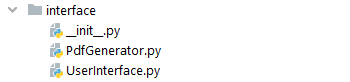
\includegraphics[width=0.85\textwidth, keepaspectratio]
                    {img/chapter4/interface_package.png}
                    \caption
                    [Zawartość pakietu \textit{interface}]
                    {Zawartość pakietu \textit{interface}}
                    \label{fig:chapter4:srodowisko_eksperymentalne:inteface_package}
                \end{minipage}
                \hfill
                \begin{minipage}[b]{0.45\textwidth}
                    \centering
                    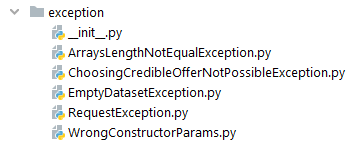
\includegraphics[width=0.85\textwidth, keepaspectratio]
                    {img/chapter4/exception_package.png}
                    \caption
                    [Zawartość pakietu \textit{exception}]
                    {Zawartość pakietu \textit{exception}}
                    \label{fig:chapter4:srodowisko_eksperymentalne:exception_package}
                \end{minipage}
            \end{figure}

            \begin{figure}[H]
                \centering
                \begin{minipage}[b]{0.45\textwidth}
                    \centering
                    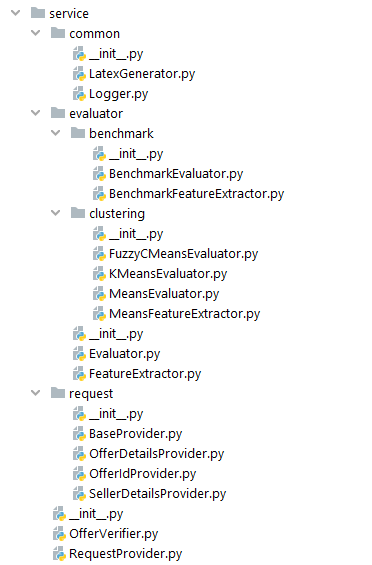
\includegraphics[width=0.85\textwidth, keepaspectratio]
                    {img/chapter4/service_package.png}
                    \caption
                    [Zawartość pakietu \textit{service}]
                    {Zawartość pakietu \textit{service}}
                    \label{fig:chapter4:srodowisko_eksperymentalne:service_package}
                \end{minipage}
                \hfill
                \begin{minipage}[b]{0.45\textwidth}
                    \centering
                    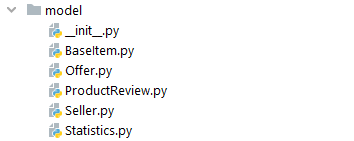
\includegraphics[width=0.85\textwidth, keepaspectratio]
                    {img/chapter4/model_package.png}
                    \caption
                    [Zawartość pakietu \textit{model}]
                    {Zawartość pakietu \textit{model}}
                    \label{fig:chapter4:srodowisko_eksperymentalne:model_package}
                \end{minipage}
            \end{figure}

            Opis plików przedstawionych na rysunku
            \ref{fig:chapter4:srodowisko_eksperymentalne:inteface_package}
        % @formatter:off
            \begin{itemize}[noitemsep,topsep=1pt]
                \item \textbf{PdfGenerator.py} - Generowanie raportów w formacie pdf
                \item \textbf{UserInterface.py} - Obsługa konsolowego interfejsu użytkownika
            \end{itemize}
        % @formatter:on

            Opis plików przedstawionych na rysunku
            \ref{fig:chapter4:srodowisko_eksperymentalne:exception_package}
        % @formatter:off
            \begin{itemize}[noitemsep,topsep=1pt]
                \item \textbf{ArraysLengthNotEqualException.py} - Klasa wyjątku informująca o nierównej długości tablicy
                \item \textbf{ChoosingCredibleOfferNotPossibleException.py} - Klasa wyjątku informująca braku możliwości wyboru wiarygodnych ofert
                \item \textbf{EmptyDatasetException.py} - Klasa wyjątku informująca o pustym zbiorze danych
                \item \textbf{RequestException.py} - Klasa wyjątku informująca o błędzie w przetwarzania żadania HTTP
                \item \textbf{WrongConstructorParamsException.py} - Klasa wyjątku informująca o błednych parametrach konstruktora
            \end{itemize}
        % @formatter:on

            Opis plików przedstawionych na rysunku
            \ref{fig:chapter4:srodowisko_eksperymentalne:service_package}
        % @formatter:off
            \begin{itemize}[noitemsep,topsep=1pt]
                \item \textbf{LatexGenerator.py} - Generowanie raportów w składni technologii LaTex
                \item \textbf{Logger.py} - Logowanie
                \item \textbf{BenchmarkEvaluator.py} - Implementacja metody z literatury
                \item \textbf{BenchmarkFeatureExtractor.py} - Ekstracja cech dla metody z literatury
                \item \textbf{FuzzyCMeansEvaluator.py} - Implementacja autorskiej metody z wykorzystaniem algorytmu C-Means
                \item \textbf{KMeansEvaluator.py} - Implementacja autorskiej metody z wykorzystaniem algorytmu K-Means
                \item \textbf{MeansEvaluator.py} - Klasa bazowa dla \textit{FuzzyCMeansEvaluator.py} oraz \textit{KMeansEvaluator.py}
                \item \textbf{MeansFeatureExtractor.py} - Ekstracja cech dla autorskiej metody
                \item \textit{Evaluator.py} - Klasa bazowa dla \textit{MeansEvaluator.py} oraz \textit{BenchmarkEvaluator.py}
                \item \textbf{FeatureExtractor.py} - Klasa bazowa dla \textit{MeansFeatureExtractor.py} oraz \textit{BenchmarkFeatureExtractor.py}
                \item \textbf{BaseProvider.py} - Klasa bazowa dla serwisów pobierających informacje o ofercie
                \item \textbf{OfferDetailsProvider.py} - Implementacja pobierania danych o ofercie
                \item \textbf{OfferIdProvider.py} - Implementacja pobierania identyfikatorów ofert dla wyszukiwanej frazy
                \item \textbf{SellerDetailsProvider.py} - Implementacja pobierania danych o sprzedawcy
                \item \textbf{OfferVerifier.py} - Implementacja weryfikacji wiarygodności ofert
                \item \textbf{RequestProvider.py} - Klasa agregująca funkjonalności\textit{OfferDetailsProvider.py}, \textit{OfferIdProvider.py}, \textit{SellerDetailsProvider.py}
            \end{itemize}
        % @formatter:on

            Opis plików przedstawionych na rysunku
            \ref{fig:chapter4:srodowisko_eksperymentalne:model_package}
        % @formatter:off
            \begin{itemize}[noitemsep,topsep=1pt]
                \item \textbf{BaseItem.py} - Klasa bazowa zawierająca unikalny identyfikator
                \item \textbf{Offer.py} - klasa modelu reprezentująca ofertę
                \item \textbf{OffersWrapper.py} - klasa modelu zapewniająca możliwość serializacji ofert do formatu \textit{.json}
                \item \textbf{ProductReview.py} - klasa modelu reprezentująca recenzję oferty
                \item \textbf{Seller.py} - klasa modelu reprezentująca sprzedawcę
                \item \textbf{Statistics.py} - klasa modelu reprezentująca statystyki generowane przez program
            \end{itemize}
        % @formatter:on

            \begin{figure}[H]
                \centering
                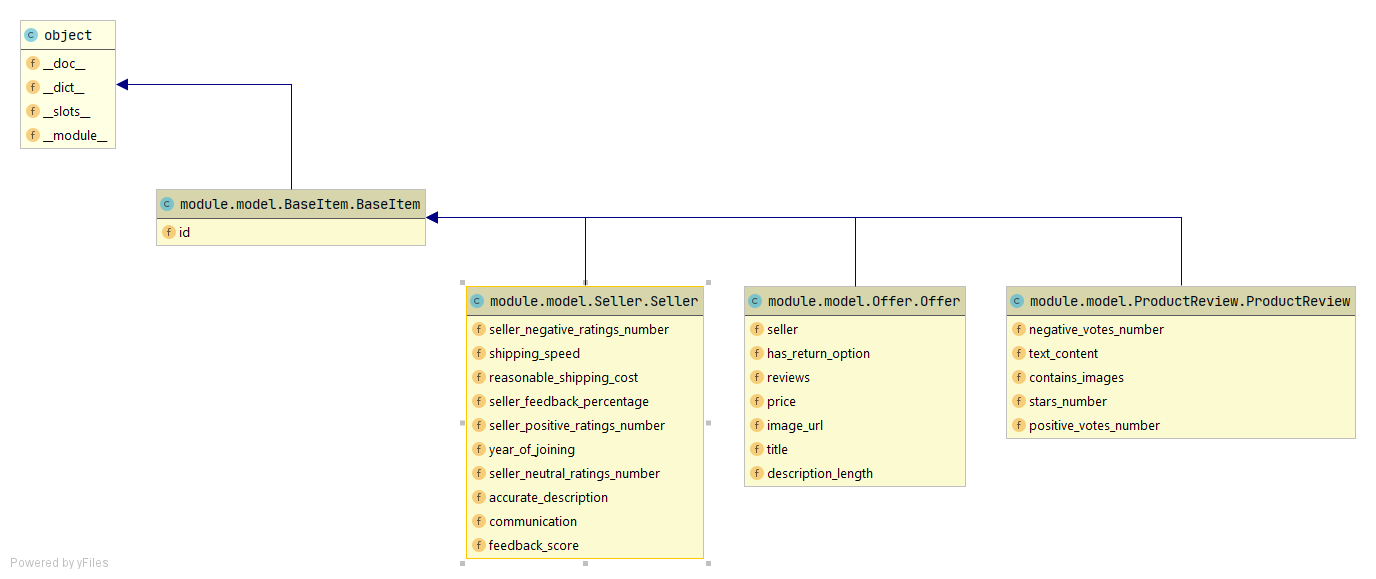
\includegraphics
                [width=\textwidth,keepaspectratio]
                {img/chapter4/model.png}
                \caption
                [Diagram UML klas zawartych w pakiecie model z pominięciem
                    \textit{Statistics}]
                {Diagram UML klas zawartych w pakiecie model z pominięciem
                    \textit{Statistics}}
                \label
                {fig:chapter4:srodowisko_eksperymentalne:model_uml}
            \end{figure}

        }
    }

    \section{Nałożone ograniczenia}
    \label{chapter4:srodowisko_eksperymentalne:ograniczenia} {
        W~ramach realizacji implementacji autorskiej metody powstał program, w~którym
        zostały nałożone pewne ograniczenia. Zostały one przedstawione poniżej:
    % @formatter:off
        \begin{itemize}[noitemsep,topsep=1pt]
            \item wymagany jest dostęp do sieci Internet
            \item program pobiera oferty tylko produktów oznaczone jako nowe
            \item program realizuje funkcjonalności tylko dla produktów katalogowych,
            nie ma możliwości analizy ofert z~produktami unikalnymi jak dzieła sztuki
            \item forma zakupu jest ograniczona do \textit{Kup Teraz} (ang. Buy Now)
            \item obsługiwana waluta to Dolar amerykański (USD)
            \item językiem w~jakim obsługiwana jest analiza treści recenzji jest
            język angielski
        \end{itemize}
    % @formatter:on
    }

    \section{Wstępne przygotowanie danych oraz ekstrakcja cech}
    \label{chapter4:srodowisko_eksperymentalne:preprocessing} {
        Wyselekcjonowane informacje, które są pobierane przez program, poddawane są
        procesowi mapowanie na klasy modelu przedstawione w~sekcji
        \ref{chapter4:srodowisko_eksperymentalne:impl_programu:struktura}. Instancja
        klasy \textit{Offer} agreguje w~sobie instancję klasy \textit{Seller} oraz listę
        instancji klasy \textit{Review}. Wskutek tego otrzymujemy obiekt z~danymi, na
        którym operuję program. Przed przekazaniem tych danych do opracowanej metody
        jest dokonywane utworzenie obiektu klasy \textit{DataFrame} dostępnego
        w~bibliotece \textit{Pandas} przedstawionej w~sekcji
        \ref{chapter4:srodowisko_eksperymentalne:impl_programu:bib:pandas}. Do tego
        obiektu w~pierwszym kroku trafiają następujące cechy oferty, przedstawione
        poniżej:

    % @formatter:off
        \begin{itemize}[noitemsep,topsep=1pt]
            \item cena produktu \textit{(offer.price)}
            \item czy istnieje możliwość zwrotu produkty \textit{(offer.has\_return\_option)}
            \item liczba liter w opisie przedstawionej ofercie
            \textit{(offer.description\_length)}
            \item liczba punktów uzyskanych na podstawie przeprowadzonych transakcji
            i~informacji zwrotnych od klientów \textit{(offer.seller.feedback\_score)}
            \item procent informacji zwrotnych od klientów o~charakterze pozytywny dla
            danego sprzedawcy \textit{(offer.seller.seller\_feedback\_percentage)}
            \item data dołączenia sprzedawcy \textit{(offer.seller.year\_of\_joining)}
            \item bezwzględna liczba pozytywnych ocen sprzedawcy
            \textit{(offer.seller.seller\_positive\_ratings\_number)}
            \item bezwzględna liczba neutralnych ocen sprzedawcy
            \textit{(offer.seller.seller\_neutral\_ratings\_number)}
            \item bezwzględna liczba negatywnych ocen sprzedawcy
            \textit{(offer.seller.seller\_negative\_ratings\_number)}
            \item ocena dokładności opisu zamieszczonego w~ofertach danego sprzedawcy
            \textit{(offer.seller.accurate\_description)}
            \item ocena kosztu przesyłki produktów zawartych w~ofertach danego
            sprzedawcy \textit{(offer.seller.reasonable\_shipping\_cost)}
            \item ocena czasu przesyłki produktów oferowanych przez danego sprzedawcę
            \textit{(offer.seller.shipping\_speed)}
            \item ocena komunikacji ze sprzedawcą \textit{(offer.seller.communication)}
        \end{itemize}
        \bigskip
    % @formatter:on

        Następnie dla kolumn nienumerycznych jest wykonywana operacja kodowania na
        wartości numeryczne za pomocą obiektu klasy \textit{LabelEncoder} z~biblioteki
        \textit{scikit-learn}, przedstawionej w~sekcji
        \ref{chapter4:srodowisko_eksperymentalne:impl_programu:bib:sklearn}. Dzięki
        temu wspomniane cechy nienumeryczne mogą się znajdować w~wektorze cech
        i~wybrany algorytm, czy też metoda może na nich operować. Kolejny krok jest
        niezwykle ważny, gdyż jest to normalizacja wartości we wszystkich kolumnach.
        Zapewnia to przeskalowanie wartości w~danej kolumnie z~pierwotnego zakresu do
        wartości z~zakresu od \textit{0} do \textit{1}.

        W~następnym etapie dokonywana jest analiza semantyczna treści każdej z~recenzji
        danej oferty. Pierwszym jej krokiem jest weryfikacja czy zawartość tekstowa
        treści jest w~języku angielskim, zgodnie z~założeniami opisanymi w~sekcji
        \ref{chapter4:srodowisko_eksperymentalne:ograniczenia}.

        Kolejno jest wykonywane wstępne przygotowanie tekstu poprzez dokonanie kroków
        takich jak transformacja wszystkich liter do postaci małych liter, tokenizacja
        słów, usunięcie słów, które występują na stop liście lub zawierają znaki inne
        niż litery od \textit{A} do \textit{Z}. Po usunięciu wspomnianych słów
        przeprowadzana jest lematyzacji, czyli sprowadzenie słowa do jego formy
        podstawowej. Wszystkie te operacji zostały wykonane przy pomocy biblioteki
        \textit{NLTK} opisanej w~sekcji
        \ref{chapter4:srodowisko_eksperymentalne:impl_programu:bib:nltk}. Na listingu
        \ref{lst:chapter4:srodowisko_eksperymentalne:preprocessing:prepare_text}
        została przedstawiona implementacja wstępne przetwarzanie tekstu.

        \begin{code}[H]
            \lstinputlisting{../listing/chapter4/prepare_text.txt}
            \caption
            [Implementacja wstępnego przetwarzania tekstu]
            {Implementacja wstępnego przetwarzania tekstu}
            \label
            {lst:chapter4:srodowisko_eksperymentalne:preprocessing:prepare_text}
        \end{code}

        Następnie jest przeprowadzana analiza sentymentu poprzez określenie emocji za
        pomocą biblioteki \textit{NRCLex}, opisanej w~sekcji
        \ref{chapter4:srodowisko_eksperymentalne:impl_programu:bib:nrclex}. Z~uzyskanej
        listy słowników (ang. dictionary), które zawierają konkretne wartości wyliczana
        jest średnia wartość danej emocji dla każdej z~treści recenzji. Dzięki temu
        uzyskujemy uśrednione wartości emocji dla wszystkich recenzji. Co warto
        wspomnieć, biblioteka \textit{NRCLex} zwraca wartości już po procesie
        normalizacji. Z~tego powodu krok ten jest wykonywany jako ostatni, aby
        dwukrotnie nie dokonywać normalizacji. Uzyskane dziesięć wartości dla każdej
        z~ofert jest dodawane do obiektu klasy \textit{DataFrame}, który został już
        wcześniej zainicjalizowany. Na listingu
        \ref{lst:chapter4:srodowisko_eksperymentalne:preprocessing:get_emotions}
        została przedstawiona implementacja ekstrakcji emocji z~treści recenzji.

        \begin{code}[H]
            \lstinputlisting{../listing/chapter4/get_emotions_from_text_content.txt}
            \caption
            [Implementacja ekstrakcji emocji z treści recenzji]
            {Implementacja ekstrakcji emocji z treści recenzji}
            \label
            {lst:chapter4:srodowisko_eksperymentalne:preprocessing:get_emotions}
        \end{code}

        Na rysunku
        \ref{fig:chapter4:srodowisko_eksperymentalne:preprocessing:activity_diagram}
        został przedstawiony diagram czynności wykonywanych w~ramach
        wstępnego przetwarzania danych oraz ekstracji cech, które zostało opisane w~tej
        sekcji.

        \begin{figure}[H]
            \centering
            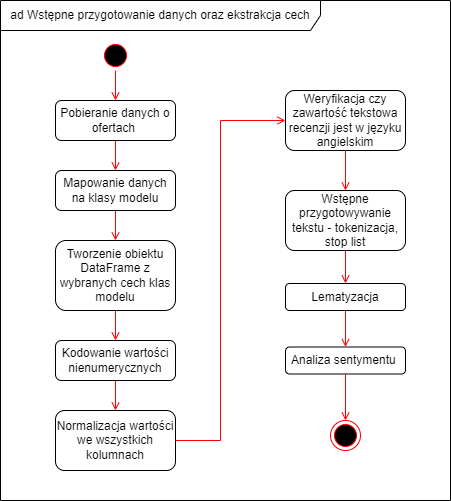
\includegraphics
            [width=0.5\textwidth,keepaspectratio]
            {img/chapter4/preprocessing_activity_diagram.drawio.png}
            \caption
            [Diagram czynności wstępnego przetwarzania danych oraz ekstracji cech]
            {Diagram czynności wstępnego przetwarzania danych oraz ekstracji cech}
            \label{fig:chapter4:srodowisko_eksperymentalne:preprocessing:activity_diagram}
        \end{figure}

    }

    \section{Implementacja autorskiej metody}
    \label{chapter4:srodowisko_eksperymentalne:impl_autorskiej_metody} {
        Zgodnie z~opisem przedstawionym w~sekcji \ref{chapter3:metoda:warianty_metody}
        autor opracował dwie bliźniacze metody, które różnią się sposobem
        klasteryzacji (grupowania). Pierwszą z~nich wykorzystuje algorytm K-Means,
        natomiast druga algorytm C-Means, ich implemetacje zostały przedstawione
        odpowiednio na listingach
        \ref{lst:chapter4:srodowisko_eksperymentalne:impl_autorskiej_metody:k_means}
        oraz
        \ref{lst:chapter4:srodowisko_eksperymentalne:impl_autorskiej_metody:c_means}.
        Do tego celu zostały wykorzystane biblioteki, w~przypadku algorytmu
        K-Means została wykorzystana biblioteka \textit{scikit-learn}, przedstawionej
        w~sekcji \ref{chapter4:srodowisko_eksperymentalne:impl_programu:bib:sklearn},
        natomiast w~drugim przypadku, jakim jest algorytm C-Means autor wykorzystał
        bibliotekę \textit{fuzzy-c-means}\cite{website:cmeans}.

        \begin{code}[H]
            \lstinputlisting{../listing/chapter4/kmeans.txt}
            \caption
            [Implementacja wykorzystująca algorytm K-Means]
            {Implementacja wykorzystująca algorytm K-Means}
            \label
            {lst:chapter4:srodowisko_eksperymentalne:impl_autorskiej_metody:k_means}
        \end{code}

        \begin{code}[H]
            \lstinputlisting{../listing/chapter4/cmeans.txt}
            \caption
            [Implementacja wykorzystująca algorytm C-Means]
            {Implementacja wykorzystująca algorytm C-Means}
            \label
            {lst:chapter4:srodowisko_eksperymentalne:impl_autorskiej_metody:c_means}
        \end{code}

        Po dokonaniu klasteryzacji są przeprowadzane kroki wspólne dla obu algorytmów,
        a~mianowicie jest to rozdzielanie obiektów klasy \textit{Offer} na dwie listy,
        ze względu na przydzielony klaster podczas grupowania. Posiadając takie dwie
        listy dokonywany jest proces wyboru klastra z~bardziej wiarygodnymi ofertami.
        Jest on oparty wartość \textit{średniej z~wszystkich ocen produktu},
        implementacja została przedstawiona na listingu
        \ref{lst:chapter4:srodowisko_eksperymentalne:impl_autorskiej_metody:credible}.
        Uzyskany w~ten sposób zbiór informacji zawiera dwie listy ofert oraz dwie
        zmienne typu boolean, zawierające wartość Prawda (ang. True) lub Fałsz (ang.
        False), odpowiednio dla każdej z~list o~tym czy ofert zawarte w~niej są
        wiarygodne, czy też nie.

        \begin{code}[H]
            \lstinputlisting{../listing/chapter4/choose_more_credible_offers.txt}
            \caption
            [Implementacja wyboru bardziej wiarygodnego klastra]
            {Implementacja wyboru bardziej wiarygodnego klastra}
            \label
            {lst:chapter4:srodowisko_eksperymentalne:impl_autorskiej_metody:credible}
        \end{code}

        Na rysunku
        \ref{fig:chapter4:srodowisko_eksperymentalne:impl_autorskiej_metody:activity_diagram}
        został przedstawiony diagram czynności wykonywanych w~czasie
        działania algorytmu autorskiej metody, które zostały opisane w~tej sekcji.

        \begin{figure}[H]
            \centering
            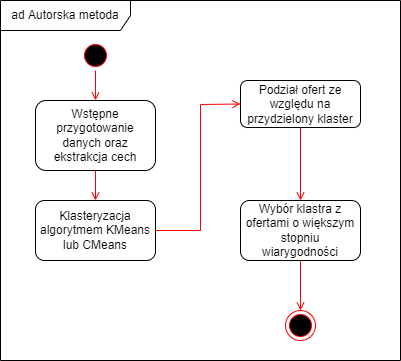
\includegraphics
            [width=0.5\textwidth,keepaspectratio]
            {img/chapter4/offer_verifier_method_activity_diagram.drawio.png}
            \caption
            [Diagram czynności autorskiej metody]
            {Diagram czynności autorskiej metody}
            \label{fig:chapter4:srodowisko_eksperymentalne:impl_autorskiej_metody:activity_diagram}
        \end{figure}

    }

    \section{Implementacja wybranej metody z~literatury}
    \label{chapter4:srodowisko_eksperymentalne:impl_literaturowej_metody} {
        Do porównania autorskiej metody zostało wybrane rozwiązanie zaproponowane
        w~artykule, opisane w~sekcji \ref{chapter2:przeglad_literatury:artykul_1}. Wybór
        ten został podyktowany faktem, że zbiór dostępnych i~wykorzystywanych
        informacji na temat oferty charakteryzuję się bardzo wysokim podobieństwem
        między dwiema metodami. Dzięki temu była możliwość bezpośredniego porównania
        na ofertach z~portali ogłoszeniowych celem uzyskania możliwie jak najbardziej
        wiarygodnych wyników badań.

        Pierwszym krokiem, jaki jest wykonywany, jest określenie czy podana wartość
        numeryczna ma odzwierciedlenie w~znaczeniu semantycznym tekstu, a~szczególnie
        w~tym, czy opinia jest pozytywna, czy negatywna. Jest to dokonywane poprzez
        sprowadzenie wartości numerycznych do zakresu od \textit{0} do \textit{1},
        następnie w~wyniku analizy semantycznej uzyskuje wynik w~jakim stopniu tekst
        ten jest pozytywny lub negatywny. Mając ten wynik, sprowadzany jest on też do
        zakresu od \textit{0} do \textit{1}. Na podstawie porównania uzyskanych
        wartości jest podejmowana decyzja czy opinia ta trafia do dalszej analizy.
        Współczynniki do porównywania wspomnianych wartości są parametryzowalne, dzięki
        czemu istnieje możliwość dopasowania celem uzyskania lepszych wyników.
        Następnie dla każdej z~ofert wyliczana jest średnia z~wartości numerycznych
        opinii, które trafiły do dalszej analizy. Implementacja przedstawionych kroków
        została przedstawiona na listingu
        \ref{lst:chapter4:srodowisko_eksperymentalne:impl_literaturowej_metody:extractor}.

        Drugim krokiem jest wykonanie operacji w~algorytmie, którego celem jest podział
        ofert na te wiarygodne oraz te niezasługujące na zaufania. Jest to dokonywane
        poprzez rozdział ofert na dwie grupy, na podstawie porównania wartości
        numerycznej z~parametryzowanym progiem. Próg ten można dostosowywać do
        wybranego zbioru danych celem uzyskania możliwie jak najlepszych wyników.
        Wspomniana wartość numeryczna jest średnia opinii wyliczoną w~kroku pierwszym
        dla każdej z~ofert. Uzyskane tak wyniki można przekazać użytkownikowi w~celu
        rekomendacji lub odradzenia przeprowadzania transakcji.

        \begin{code}[H]
            \lstinputlisting{../listing/chapter4/benchmark_feature_extractor.txt}
            \caption
            [Implementacja algorytmu weryfikacji zgodności wartości numerycznej z
            wynikiem analizy semantycznej]
            {Implementacja algorytmu weryfikacji zgodności wartości numerycznej z
            wynikiem analizy semantycznej}
            \label
            {lst:chapter4:srodowisko_eksperymentalne:impl_literaturowej_metody:extractor}
        \end{code}

        \begin{code}[H]
            \lstinputlisting{../listing/chapter4/benchmark_evaluator.txt}
            \caption
            [Implementacja algorytmu oceny wiarygodności ofert na podstawie ocen]
            {Implementacja algorytmu oceny wiarygodności ofert na podstawie ocen}
            \label
            {lst:chapter4:srodowisko_eksperymentalne:impl_literaturowej_metody:evaluator}
        \end{code}

    }

    \section{Maszyna wykorzystywana do eksperymentów}
    \label{chapter4:srodowisko_eksperymentalne:maszyna} {
        Do przeprowadzenia eksperymentów został wykorzystany komputer stacjonarny
        o~specyfikacji przedstawione w~tabeli
        \ref{tab:chapter4:srodowisko_eksperymentalne:maszyna:specyfikacja}. Systemem
        operacyjnym, jaki został wykorzystany na wspomnianej maszynie był
        \textit{Microsoft Windows 10 Pro}\cite{website:windows} w~wersji
        \textit{10.0.19042 N/A Build 19042} o~architekturze 64-bitowej.

        \begin{table}[H]
			\footnotesize
            \centering
            \begin{tabular}{|c|c|}
                \hline
                Płyta główna & Gigabyte GA-EP45-DS4 \\ \hline
                Procesor & Intel(R) Core(TM)2 Duo CPU E8400 @ 3.00GHz 2.67 GHz \\ \hline
                Karta graficzna & NVIDIA GEFORCE GT 640 \\ \hline
                Pamięć RAM & DDR2 Kingston 8GB 800mhz \\ \hline
                Dysk twardy & Kingston SATA SSD A400 240GB 2,5" \\ \hline
            \end{tabular}
            \caption
            [Specyfikacja maszyny do wykonywania eksperymentów]
            {Specyfikacja maszyny do wykonywania eksperymentów}
            \label{tab:chapter4:srodowisko_eksperymentalne:maszyna:specyfikacja}
        \end{table}
    }

    \section{Zbiory danych wykorzystane do badań}
    \label{chapter4:srodowisko_eksperymentalne:zbiory_danych} {
        W~ramach przeprowadzonych badań, przedstawionych w~rozdziale
        \ref{chapter5:eksperymenty} zostały wybrane zbiory dane do eksperymentów.
        Zostały one stworzone na podstawie ofert z~portalu eBay\cite{website:ebay}.

        Portal ten w~dosyć specyficzny i~nie do końca konsekwentny sposób wyświetla
        dodawane opinie. Pomimo faktu wyszukiwania jednego, konkretnego i~nowego
        produktu katalogowego, część ofert ma dokładnie takie same opinie, pomimo że są
        od innych sprzedawców. Niestety nie jest to wykonane konsekwentnie, gdyż można
        zauważyć pewne podgrupy ofert współdzielące te opinie, niektóre oferty mają
        opinie niepowtarzające się nigdzie indziej. Ze względu na fakt, że jednym
        z~głównych elementów, jakie są analizowane są opinie autor niniejszej pracy
        zdecydował, że wybieranie do zbioru danych ofert z~dokładnie takimi samymi
        oferta nie jest sensowne. Zdecydował on aby z~każdej grupy ofert gdzie
        powtarzają się opinie wybrać zaledwie po dwie do trzech ofert.

        Co więcej, taki zabieg pomoga przy przeprowadzaniu badań ponieważ każdą z~ofert
        musi ocenić człowiek aby możliwa była weryfikacja skuteczności. W~przypadku
        zbiorów danych zawierających np. setki ofert jest to proces bardzo czasochłonny
        i~żmudny. Oczywiście w~przypadku realnego użycia metody nie trzeba wykonywać
        ręcznej oceny każdej oferty więc bez problemu można dokonywać weryfikacji setek
        ofert.

        Z~obserwacji autora niniejszej pracy wynika, że na tym portalu większość ofert
        produktów katalogowych ma pozytywne opinie. W~przypadku wykorzystanych zbiorów
        danych opinie również są głównie pozytywne, co wpływa, że ich średnia jest
        zbliżona do wartości \textit{4.5}. Nie mniej została podjęta decyzja
        o~korzystaniu z~tej cechy, gdyż w~założeniach algorytmu jest to jedna
        z~ważniejszych cech. Tym bardziej że metoda literaturowa wykorzystuję tę
        wartość do określania czy opinia jest wiarygodna. W~poniższych sekcjach została
        przedstawiona charakterystyka każdego ze zbiorów.

        \subsection{Zbiór danych \#1}
        \label{chapter4:srodowisko_eksperymentalne:zbiory_danych:1} {

            \begin{table}[H]
                \scriptsize
                \centering
                \begin{tabular}{|c|c|}
                    \hline
                    Nazwa & Wartość \\ \hline
                    Nazwa katalogowa & Logitech m330 silent plus wireless mouse \\ \hline
                    Liczba ofert & 11 \\ \hline
                    Liczba ofert określona jako wiarygodna przez eksperta & 5 \\ \hline
                    Liczba ofert określona jako niewiarygodna przez eksperta & 6 \\ \hline
                \end{tabular}
                \caption
                [Podstawowe informacje o zbiorze danych \#1]
                {Podstawowe informacje o zbiorze danych \#1}
                \label{Logitech m330 silent plus wireless mouse}
            \end{table}

            \begin{figure}[H]
                \centering
                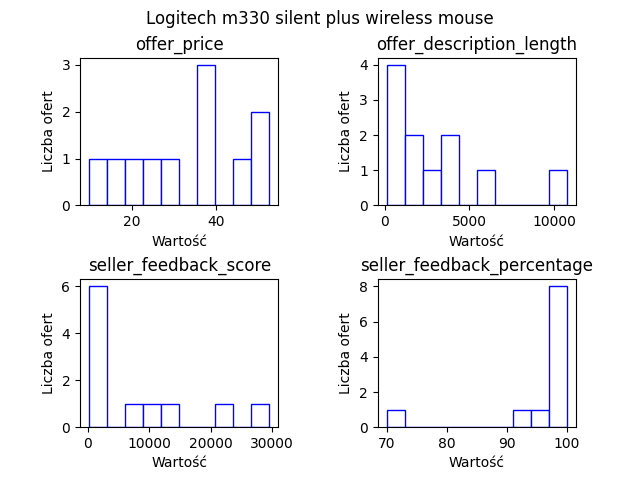
\includegraphics
                [width=0.85\textwidth,keepaspectratio]
                {img/chapter4/dataset1/Logitechm330silentpluswirelessmouse_1.png}
                \caption
                [Histogramy wybranych cech oferty dla zbioru danych \#1, cz. 1]
                {Histogramy wybranych cech oferty dla zbioru danych \#1, cz. 1}
                \label{fig:chapter4:srodowisko_eksperymentalne:zbiory_danych:1:1}
            \end{figure}

            \begin{figure}[H]
                \centering
                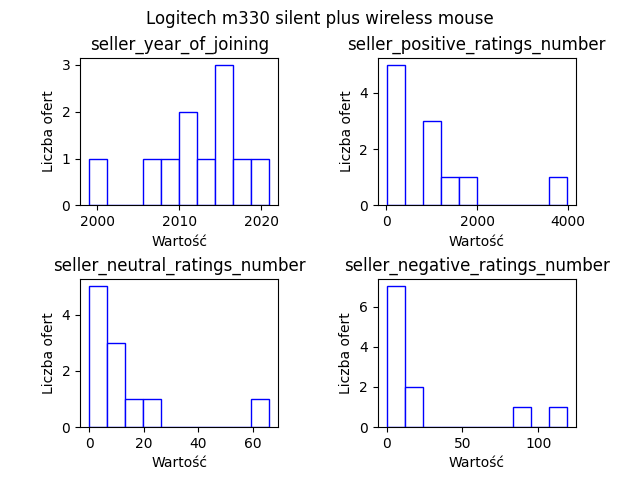
\includegraphics
                [width=0.85\textwidth,keepaspectratio]
                {img/chapter4/dataset1/Logitechm330silentpluswirelessmouse_2.png}
                \caption
                [Histogramy wybranych cech oferty dla zbioru danych \#1, cz. 2]
                {Histogramy wybranych cech oferty dla zbioru danych \#1, cz. 2}
                \label{fig:chapter4:srodowisko_eksperymentalne:zbiory_danych:1:2}
            \end{figure}

            \begin{figure}[H]
                \centering
                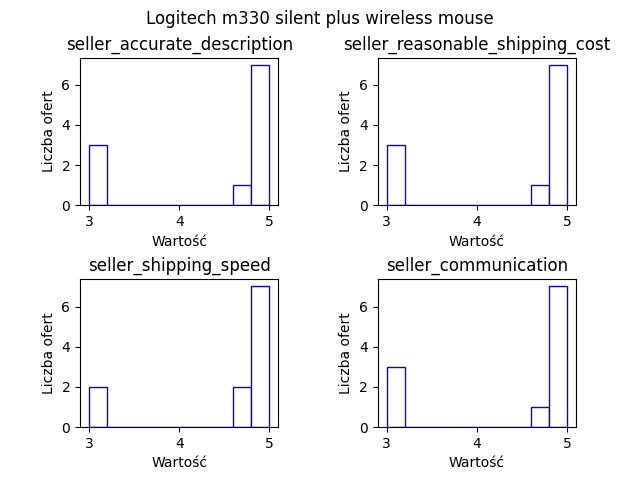
\includegraphics
                [width=0.85\textwidth,keepaspectratio]
                {img/chapter4/dataset1/Logitechm330silentpluswirelessmouse_3.png}
                \caption
                [Histogramy wybranych cech oferty dla zbioru danych \#1, cz. 3]
                {Histogramy wybranych cech oferty dla zbioru danych \#1, cz. 3}
                \label{fig:chapter4:srodowisko_eksperymentalne:zbiory_danych:1:3}
            \end{figure}

            \begin{figure}[H]
                \centering
                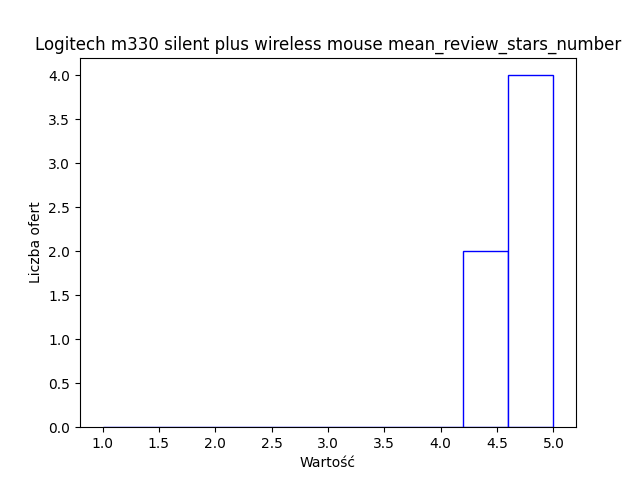
\includegraphics
                [width=0.5\textwidth,keepaspectratio]
                {img/chapter4/dataset1/Logitechm330silentpluswirelessmouse_mean_review_stars_number.png}
                \caption
                [Histogram średniej wartości oceny dla oferty, zbiór danych \#1]
                {Histogram średniej wartości oceny dla oferty, zbiór danych \#1}
                \label{fig:chapter4:srodowisko_eksperymentalne:zbiory_danych:1:4}
            \end{figure}
        }

        \subsection{Zbiór danych \#2}
        \label{chapter4:srodowisko_eksperymentalne:zbiory_danych:2} {

            \begin{table}[H]
                \scriptsize
                \centering
                \begin{tabular}{|c|c|}
                    \hline
                    Nazwa & Wartość \\ \hline
                    Nazwa katalogowa & Dell kb522 \\ \hline
                    Liczba ofert & 16 \\ \hline
                    Liczba ofert określona jako wiarygodna przez eksperta & 9 \\ \hline
                    Liczba ofert określona jako niewiarygodna przez eksperta & 7 \\ \hline
                \end{tabular}
                \caption
                [Podstawowe informacje o zbiorze danych \#2]
                {Podstawowe informacje o zbiorze danych \#2}
                \label{Dell kb522}
            \end{table}

            \begin{figure}[H]
                \centering
                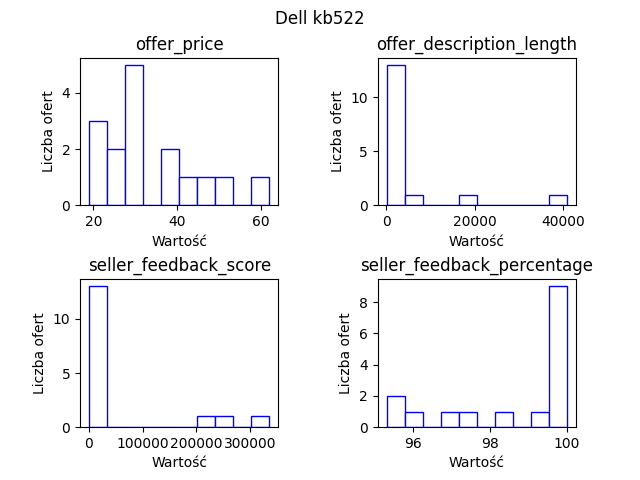
\includegraphics
                [width=0.85\textwidth,keepaspectratio]
                {img/chapter4/dataset2/Dellkb522_1.png}
                \caption
                [Histogramy wybranych cech oferty dla zbioru danych \#2, cz. 1]
                {Histogramy wybranych cech oferty dla zbioru danych \#2, cz. 1}
                \label{fig:chapter4:srodowisko_eksperymentalne:zbiory_danych:2:1}
            \end{figure}

            \begin{figure}[H]
                \centering
                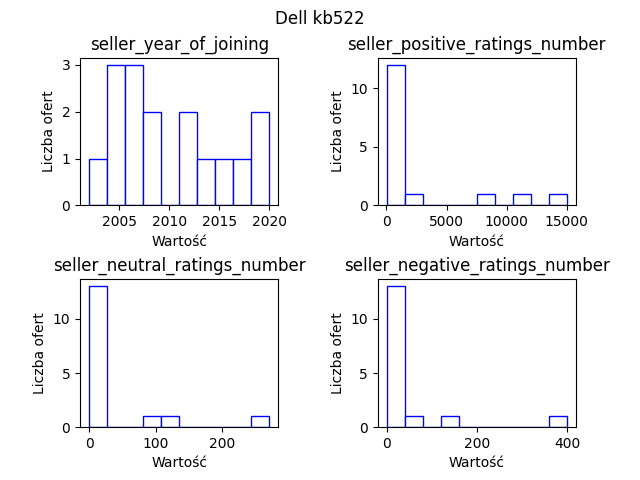
\includegraphics
                [width=0.85\textwidth,keepaspectratio]
                {img/chapter4/dataset2/Dellkb522_2.png}
                \caption
                [Histogramy wybranych cech oferty dla zbioru danych \#2, cz. 2]
                {Histogramy wybranych cech oferty dla zbioru danych \#2, cz. 2}
                \label{fig:chapter4:srodowisko_eksperymentalne:zbiory_danych:2:2}
            \end{figure}

            \begin{figure}[H]
                \centering
                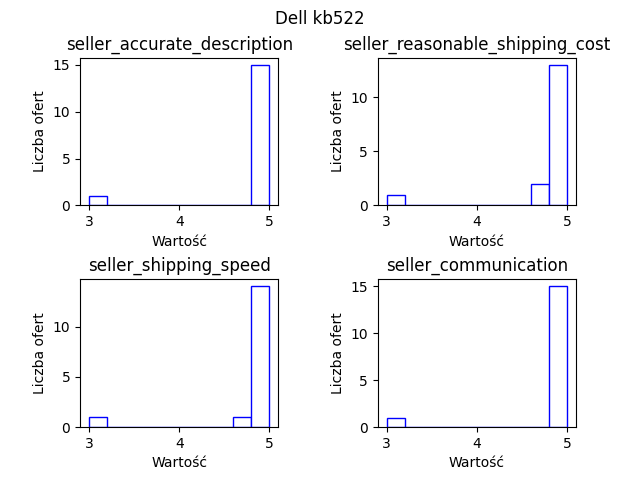
\includegraphics
                [width=0.85\textwidth,keepaspectratio]
                {img/chapter4/dataset2/Dellkb522_3.png}
                \caption
                [Histogramy wybranych cech oferty dla zbioru danych \#2, cz. 3]
                {Histogramy wybranych cech oferty dla zbioru danych \#2, cz. 3}
                \label{fig:chapter4:srodowisko_eksperymentalne:zbiory_danych:2:3}
            \end{figure}

            \begin{figure}[H]
                \centering
                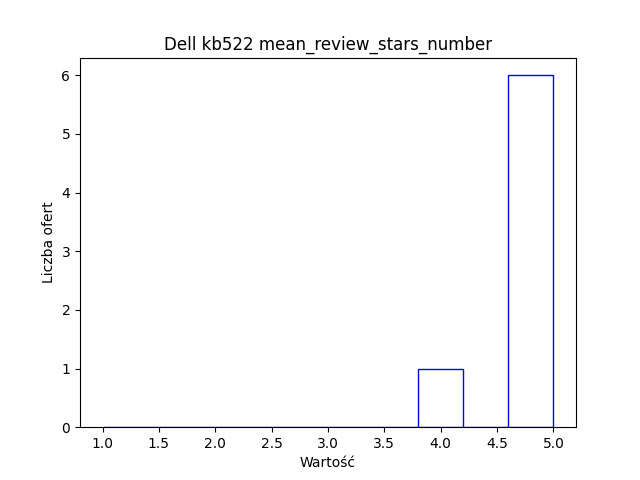
\includegraphics
                [width=0.5\textwidth,keepaspectratio]
                {img/chapter4/dataset2/Dellkb522_mean_review_stars_number.png}
                \caption
                [Histogram średniej wartości oceny dla oferty, zbiór danych \#2]
                {Histogram średniej wartości oceny dla oferty, zbiór danych \#2}
                \label{fig:chapter4:srodowisko_eksperymentalne:zbiory_danych:2:4}
            \end{figure}
        }

        \subsection{Zbiór danych \#3}
        \label{chapter4:srodowisko_eksperymentalne:zbiory_danych:3} {

            \begin{table}[H]
                \scriptsize
                \centering
                \begin{tabular}{|c|c|}
                    \hline
                    Nazwa & Wartość \\ \hline
                    Nazwa katalogowa & Apple iPhone 11 128gb \\ \hline
                    Liczba ofert & 21 \\ \hline
                    Liczba ofert określona jako wiarygodna przez eksperta & 10 \\ \hline
                    Liczba ofert określona jako niewiarygodna przez eksperta & 11 \\ \hline
                \end{tabular}
                \caption
                [Podstawowe informacje o zbiorze danych \#3]
                {Podstawowe informacje o zbiorze danych \#3}
                \label{Apple iPhone 11 128gb}
            \end{table}

            \begin{figure}[H]
                \centering
                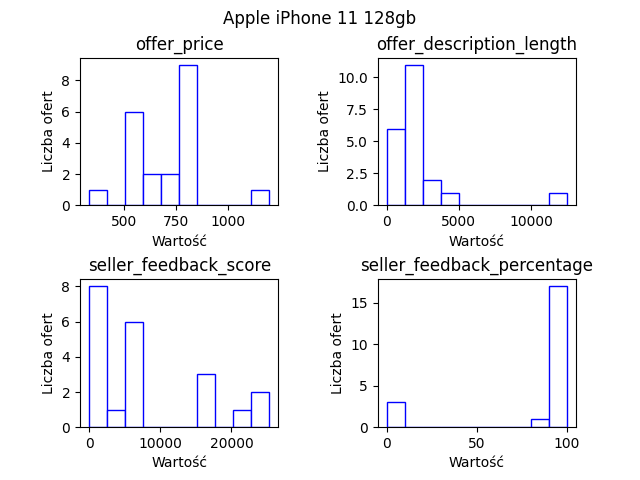
\includegraphics
                [width=0.85\textwidth,keepaspectratio]
                {img/chapter4/dataset3/AppleiPhone11128gb_1.png}
                \caption
                [Histogramy wybranych cech oferty dla zbioru danych \#3, cz. 1]
                {Histogramy wybranych cech oferty dla zbioru danych \#3, cz. 1}
                \label{fig:chapter4:srodowisko_eksperymentalne:zbiory_danych:3:1}
            \end{figure}

            \begin{figure}[H]
                \centering
                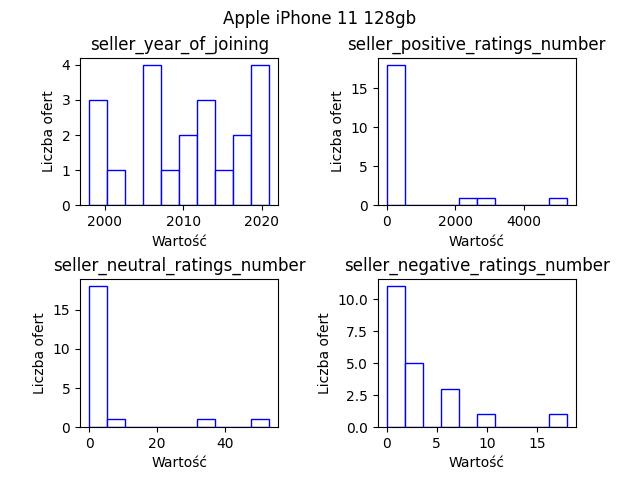
\includegraphics
                [width=0.85\textwidth,keepaspectratio]
                {img/chapter4/dataset3/AppleiPhone11128gb_2.png}
                \caption
                [Histogramy wybranych cech oferty dla zbioru danych \#3, cz. 2]
                {Histogramy wybranych cech oferty dla zbioru danych \#3, cz. 2}
                \label{fig:chapter4:srodowisko_eksperymentalne:zbiory_danych:3:2}
            \end{figure}

            \begin{figure}[H]
                \centering
                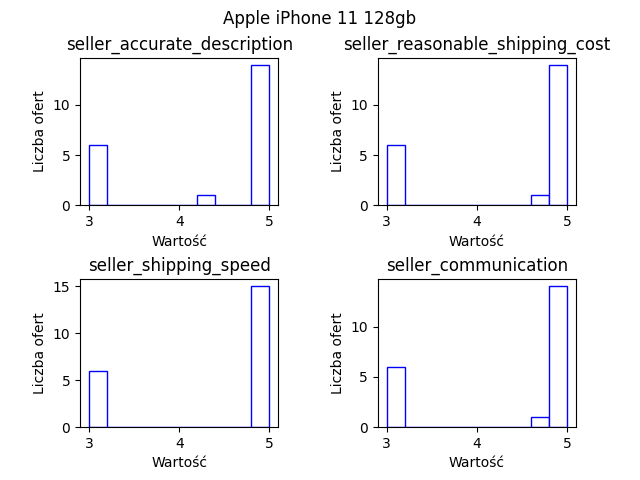
\includegraphics
                [width=0.85\textwidth,keepaspectratio]
                {img/chapter4/dataset3/AppleiPhone11128gb_3.png}
                \caption
                [Histogramy wybranych cech oferty dla zbioru danych \#3, cz. 3]
                {Histogramy wybranych cech oferty dla zbioru danych \#3, cz. 3}
                \label{fig:chapter4:srodowisko_eksperymentalne:zbiory_danych:3:3}
            \end{figure}

            \begin{figure}[H]
                \centering
                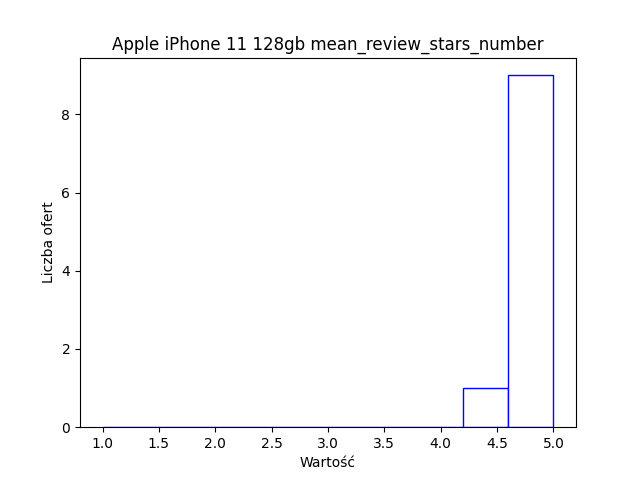
\includegraphics
                [width=0.5\textwidth,keepaspectratio]
                {img/chapter4/dataset3/AppleiPhone11128gb_mean_review_stars_number.png}
                \caption
                [Histogram średniej wartości oceny dla oferty, zbiór danych \#3]
                {Histogram średniej wartości oceny dla oferty, zbiór danych \#3}
                \label{fig:chapter4:srodowisko_eksperymentalne:zbiory_danych:3:4}
            \end{figure}
        }

        \subsection{Zbiór danych \#4}
        \label{chapter4:srodowisko_eksperymentalne:zbiory_danych:4} {

            \begin{table}[H]
                \scriptsize
                \centering
                \begin{tabular}{|c|c|}
                    \hline
                    Nazwa & Wartość \\ \hline
                    Nazwa katalogowa & Logitech m185 \\ \hline
                    Liczba ofert & 16 \\ \hline
                    Liczba ofert określona jako wiarygodna przez eksperta & 5 \\ \hline
                    Liczba ofert określona jako niewiarygodna przez eksperta & 11 \\
                    \hline
                \end{tabular}
                \caption
                [Podstawowe informacje o zbiorze danych \#4]
                {Podstawowe informacje o zbiorze danych \#4}
            \end{table}

            \begin{figure}[H]
                \centering
                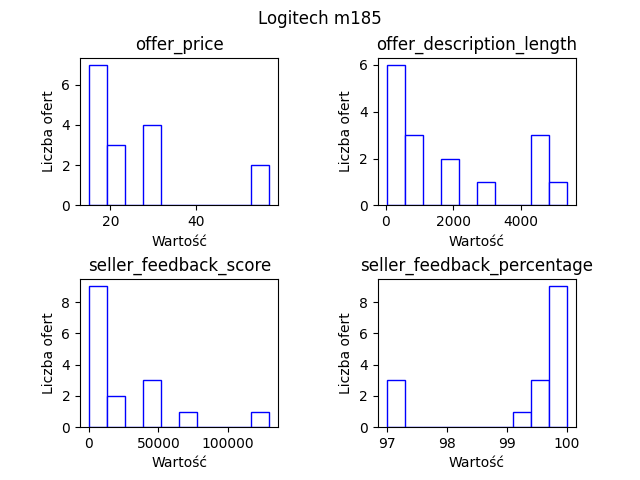
\includegraphics
                [width=0.85\textwidth,keepaspectratio]
                {img/chapter4/dataset4/Logitechm185_1.png}
                \caption
                [Histogramy wybranych cech oferty dla zbioru danych \#4, cz. 1]
                {Histogramy wybranych cech oferty dla zbioru danych \#4, cz. 1}
                \label{fig:chapter4:srodowisko_eksperymentalne:zbiory_danych:4:1}
            \end{figure}

            \begin{figure}[H]
                \centering
                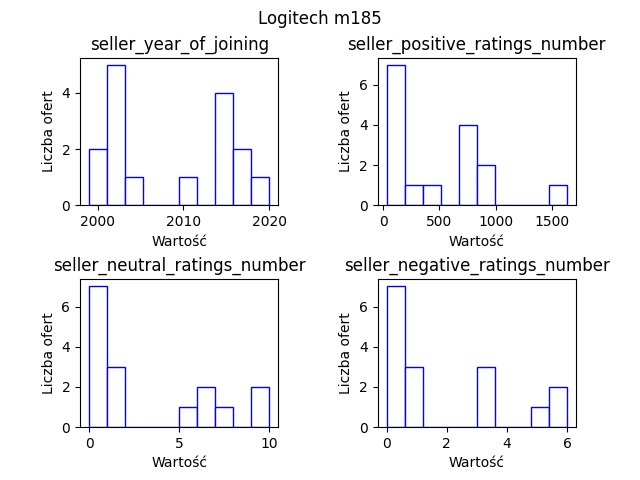
\includegraphics
                [width=0.85\textwidth,keepaspectratio]
                {img/chapter4/dataset4/Logitechm185_2.png}
                \caption
                [Histogramy wybranych cech oferty dla zbioru danych \#4, cz. 2]
                {Histogramy wybranych cech oferty dla zbioru danych \#4, cz. 2}
                \label{fig:chapter4:srodowisko_eksperymentalne:zbiory_danych:4:2}
            \end{figure}

            \begin{figure}[H]
                \centering
                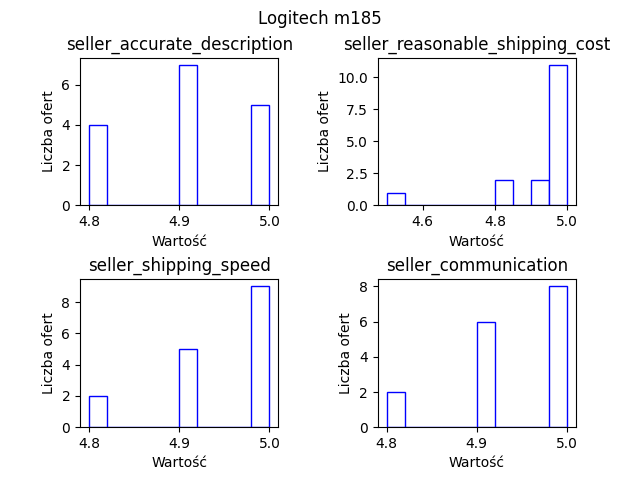
\includegraphics
                [width=0.85\textwidth,keepaspectratio]
                {img/chapter4/dataset4/Logitechm185_3.png}
                \caption
                [Histogramy wybranych cech oferty dla zbioru danych \#4, cz. 3]
                {Histogramy wybranych cech oferty dla zbioru danych \#4, cz. 3}
                \label{fig:chapter4:srodowisko_eksperymentalne:zbiory_danych:4:3}
            \end{figure}

            \begin{figure}[H]
                \centering
                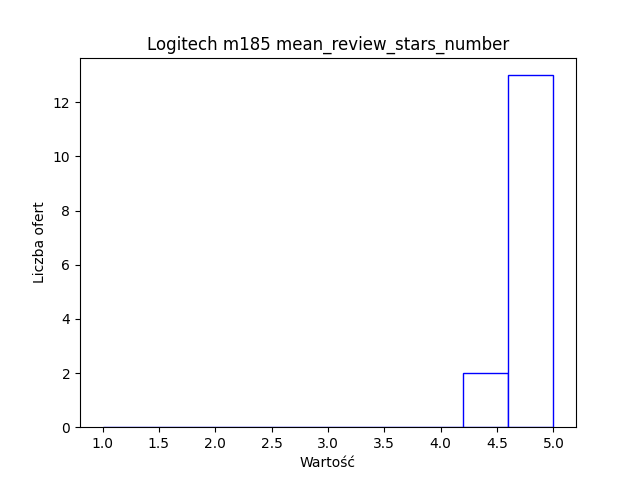
\includegraphics
                [width=0.5\textwidth,keepaspectratio]
                {img/chapter4/dataset4/Logitechm185_mean_review_stars_number.png}
                \caption
                [Histogram średniej wartości oceny dla oferty, zbiór danych \#4]
                {Histogram średniej wartości oceny dla oferty, zbiór danych \#4}
                \label{fig:chapter4:srodowisko_eksperymentalne:zbiory_danych:4:4}
            \end{figure}
        }

        \subsection{Znaczące różnice między zbiorami danych}
        \label{chapter4:srodowisko_eksperymentalne:zbiory_danych:roznice} {
            Jedną z~ciekawych obserwacji jest to, że w~przypadku zbiorów \#2 oraz \#4
            istnieją wartości \textit{seller\_feedback\_score}, które są stukrotnie
            większe w~porównaniu do tych występujących w~zbiorach \#1 oraz \#3.

            Co więcej, w~przypadku zbiorów \#2 oraz \#4 wartości
            \textit{seller\_feedback\_percentage} występują w~bardzo wąskim zakresie od
            około 95 do 100 natomiast w~pozostałych zbiorach mamy duży szerszy zakres
            wartości.

            Warto też zwrócić uwagę na zbiór \#4 gdzie wartości
            \textit{seller\_accurate\_description},
            \textit{seller\_reasonable\_shipping\_cost}, \textit{seller\_shipping\_speed},
            \textit{seller\_communication} są tylko z~wysokiego przedziału, czyli
            głównie od 4,8 do 5. Pozostałe zbiory posiadają dla tych pól również
            mniejsze wartości.
        }

    }

}
\end{document}
